\setAuthor{}
\setRound{lõppvoor}
\setYear{2019}
\setNumber{G 4}
\setDifficulty{4}
\setTopic{TODO}

\prob{Konveier}
Sile metallplaat pikkusega $l$ sõidab konveieril. Konveier koosneb kahest osast ning kummalgi osal on oma sile konveierilint. Mõlema lindi pikkus on $x$, kuid esimene lint liigub kiirusega $v_1$ ning teine kiirusega $v_2$. Algasendis on plaat esimese lindi alguses nii, et plaat asub täielikult esimesel konveierilindil ning plaadi tagumine serv ühtib esimese lindi algusega. Lõppasendis on plaat teise lindi lõpus nii, et plaat asub täielikult teisel konveierilindil ning plaadi esimene serv ühtib teise lindi lõpuga. Leida aeg $t$, mis kulub plaadil algasendist lõppasendisse jõudmiseks. Hõõrdetegur plaadi ja esimese konveierilindi vahel on $\mu_{1}$ ning plaadi ja teise konveierilindi vahel $\mu_{2}$. Eeldada, et üleminekukohas on vahe konveierilintide vahel tühiselt väike ning aeg, mis kulub plaadi kiiruse muutumiseks üleminekukohas, on tühiselt väike võrreldes koguajaga. 



\hint

\solu
Olles täielikult esimesel lindil, on plaadi kiirus $v_1$ ning teisel lindil $v_2$. Plaadi kiirus muutub üleminekukohas $v_1$-lt $v_2$-le, kui hõõrdejõud teise konveierilindiga ületab hõõrdejõu esimese konveierilindiga. Olgu plaadi mass $M$ ning plaadi joontihedus piki konveierit $\rho = M/l$. Piirjuhul saame hõõrdejõudude võrdsusest:
$$\mu_{1}M_1g = \mu_{2}M_2g$$
kus $M_1$ ja $M_2$ on vastavalt esimese ja teise lindi peal oleva plaadi osa massid. Olgu esimesel lindil oleva osa pikkus $l_1$ ning teisel osal $l_2$. Kasutades joontihedust saame:
$$\mu_{1} \rho l_1 g = \mu_{2}\rho l_2 g$$.
Taandades ühised kordajad saame võrrandisüsteemi:
$$\mu_{1} l_1 = \mu_{2} l_2$$
$$l_1 + l_2 = l$$
Siit saame avaldada $l_1$-e:
$$l_1 = \frac{l}{1+\frac{\mu_{1}}{\mu_{2}}}$$

\begin{center}
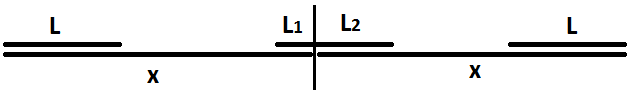
\includegraphics[scale=0.5]{2019-v3g-04-sol.png}
\end{center}


Joonisel on kujutatud plaadi algasend, lõppasend ning piirjuht, kus kiirus muutub (tühiselt väikese aja jooksul). Algasendist piirjuhuni läbib plaat vahemaa $x - l_1$ kiirusel $v_1$. Piirjuhust lõppasendini läbib plaat vahemaa $x - l_2$ kiirusel $v_2$. Seega koguaeg:
$$t = \frac{x - l_1}{v_1} + \frac{x - l_2}{v_2}$$
Asendades saame:
$$t=\frac{v_2 x - v_2 l_1 + v_1 x - v_1 l_2}{v_1 v_2} =$$
$$\frac{x(v_1 + v_2) - lv_1 - l_1 v_2 + l_1 v_1}{v_1 v_2} =$$
$$\frac{x(v_1 + v_2) - lv_1 + \frac{l(v_1 - v_2)}{1+\frac{\mu_{1}}{\mu_{2}}}}{v_1 v_2}$$
\probend